\documentclass[11pt]{article}
\usepackage[margin=1in]{geometry}
\usepackage[T1]{fontenc}
\usepackage{lmodern}
\usepackage{microtype}
\usepackage{booktabs}
\usepackage{graphicx}
\usepackage{hyperref}
\usepackage{amsmath}
\usepackage{siunitx}
\usepackage{enumitem}
\usepackage{caption}
\usepackage{subcaption}
\usepackage{url}

\title{OTShield Bench: Reproducible Measurement of OT Cyber-Detection Resilience Under Degraded Connectivity}
\author{Jayachandra Reddy Palle\\OTShield Bench project\\\url{https://github.com/ASHTHRA/otshield-bench}}
\date{Research preprint draft --- September 2026}

\newcommand{\otb}{OTShield Bench}
\newcommand{\fc}{Modbus/TCP Function Code 3}

\begin{document}
\maketitle

\begin{abstract}
Operational-technology (OT) detection benchmarks often report nominal detection
scores without preserving how the observation path behaves when network timing
degrades. We present \otb, a vendor-neutral and reproducible benchmark for
measuring detection effectiveness, resource cost, and resilience under controlled
connectivity impairment. The v0.6 study pairs a fixed 50~ms polling-burst
detector with a robust detector whose threshold was frozen from independent
historical clean evidence. In an isolated OpenPLC laboratory, the completed
replacement study evaluates 25 trials across five conditions: 125 condition runs,
7,500 planned read-only \fc{} transactions, and 250 detector evaluations. Both
detectors have mean recall/F1 of 1.0/1.0 in clean and +20~ms conditions and
0.95/0.9738 under +20~ms, 5~ms jitter, and 5\% loss. At +40~ms and 10~ms jitter,
paired robust-minus-baseline recall is 0.54 (95\% unbounded Student-$t$ interval
0.496--0.584); at +60~ms and 10~ms jitter it is 1.0. Coverage is 1.0 and false
positives are zero in every condition. These results describe one documented,
read-only isolated laboratory and timing workload. They do not establish
production validation, universal superiority, full GRFICS validation, external
replication, or industry adoption.
\end{abstract}

\section{Introduction}
OT environments combine timing, availability, safety, and process constraints
that are not captured by a nominal classifier score alone. Guidance for OT
security emphasizes these operational characteristics \cite{stouffer2023ot}, while
cross-sector guidance calls for measurable cybersecurity outcomes
\cite{cisa2023cpg}. Existing evaluations of ICS-focused detection are valuable
for measuring adversary-oriented behavior \cite{mitre2021ics}; a complementary
question is whether a detector remains reliable when the telemetry path is
delayed, jittered, lossy, or resource constrained.

This paper presents the v0.6 research package of \otb. The benchmark separates
scenario generation, telemetry normalization, detector execution, and evaluation
through versioned OTB-SCENARIO, OTB-TELEMETRY, OTB-DETECT, and OTB-EVAL
abstractions. Its central contribution is methodological: identical captured
observations are evaluated by paired detectors, calibration is frozen outside the
test study, run-level uncertainty is retained, and provenance and failures are
preserved with integrity records.

\section{Motivation and research question}
The motivating question is: \emph{under controlled degraded connectivity, how
does a fixed timing detector compare with an independently calibrated robust
timing detector when both analyze the same OT observations?} This is a bounded
measurement question, rather than a claim that one algorithm is a universally
better intrusion detector. It tests whether the benchmark can expose a difference
between complete transaction coverage and stable timing-based detection.

\section{Related work}
OT security guidance frames reliability and safety as first-class constraints
\cite{stouffer2023ot}, and CISA's performance goals provide a measurement
orientation for critical-infrastructure security \cite{cisa2023cpg}. MITRE
Engenuity's ICS evaluations provide an important adversary-behavior detection
perspective \cite{mitre2021ics}. \otb{} addresses a narrower experimental axis:
the resilience of an observation-dependent detector under network-path
impairment, with an explicit evidence boundary and reproducible artifacts. The
configured PLC image is GRFICS-derived; the upstream project is acknowledged
here \cite{formbygrfics}, but this work does not claim a completed GRFICSv3
process simulation.

\section{OTShield benchmark architecture}
The offline benchmark path emits labeled events or ingests passive observations,
applies observation faults, runs detectors, and exports metrics, configuration,
provenance, and hashes. The laboratory path is separate: a bounded client emits
read-only \fc{} traffic to an isolated OpenPLC instance, packet capture occurs in
the server network namespace, and the capture is normalized into transaction-aware
telemetry. Detector labels are cleared before prediction; ground truth remains in
the evaluation layer. A baseline and robust detector therefore receive the same
canonical observation view.

The v0.6 runner records a protocol, raw PCAP, normalized telemetry, provenance,
per-detector observations and results, and SHA-256 integrity files. A readiness
gate checks host prerequisites without creating study evidence. Lifecycle guards
hold an advisory lock through cleanup and accounting and verify the identity of
the OpenPLC container at condition boundaries.

\section{Experimental methodology}
The completed replacement study is identified by \texttt{20260922T021855Z}.
It contains 25 trials and five conditions, with 60 planned transactions per
condition. Transactions 1--20 are normal-pre, 21--40 are a controlled polling
burst, and 41--60 are normal-post. Normal spacing is approximately 100~ms and
burst spacing approximately 10~ms. The first interval is unavailable rather than
treated as a measured zero. The impairment is applied with Linux \texttt{tc
netem} on client egress; capture is at the OpenPLC/server namespace. Condition
order rotates deterministically between trials, and one OpenPLC instance serves
the five conditions within a trial.

The measured laboratory is a minimal isolated Docker-based OpenPLC setup using
the configured GRFICS-derived image. It is laboratory evidence for this workload,
not production OT validation or a full process simulation. Synthetic fixtures and
mocked tests validate software behavior but are not included as laboratory
measurements.

\begin{table}[t]
\centering
\caption{Predeclared network conditions.}
\label{tab:conditions}
\begin{tabular}{lrrr}
\toprule
Condition & Delay (ms) & Jitter (ms) & Loss (\%)\\
\midrule
Clean & 0 & 0 & 0\\
Delay20 & 20 & 0 & 0\\
Delay20/Jitter5/Loss5 & 20 & 5 & 5\\
Delay40/Jitter10 & 40 & 10 & 0\\
Delay60/Jitter10 & 60 & 10 & 0\\
\bottomrule
\end{tabular}
\end{table}

\section{Frozen calibration methodology}
The baseline alerts when $0 <$ observed interval $<50.0$~ms. The robust detector
uses the same strict inequality with a threshold frozen before v0.6 evaluation.
Only historical v0.5 clean observations that were matched, explicitly normal,
positive, and finite were eligible. The 195 eligible intervals yielded
$M=101.010009765625$~ms, $\mathrm{MAD}=0.14892578125$~ms, robust sigma
$=1.4826\times\mathrm{MAD}=0.22079736328125$~ms, and threshold
$M-3.5\times\mathrm{sigma}=100.23721899414062$~ms. No v0.6 test observation
was used. The frozen JSON and its hash are retained in the release manifest.

\section{Experimental conditions}
The burst is the only labeled anomaly and is fixed by the protocol, never by
detector output. Loss can reduce observations while timing impairment changes
arrival intervals and latency. Coverage measures observed planned transactions;
end-to-end recall accounts for planned anomalies. The five conditions vary only
the declared delay, jitter, and loss parameters. This design makes the paired
comparison interpretable while keeping the experiment within a read-only
Modbus/TCP workload.

\section{Results}
The aggregate JSON is the numerical source of truth. Mean recall and F1 are
identical for the two detectors in the first three conditions: 1.0/1.0 in clean
and Delay20, and 0.95/0.9737564284932706 in Delay20/Jitter5/Loss5. At
Delay40/Jitter10, baseline recall/F1 is 0.46/0.6230102454707571 while robust is
1.0/1.0. At Delay60/Jitter10, baseline is 0.0/0.0 while robust is 1.0/1.0.
Coverage remains 1.0 and false positives remain zero in all conditions.

\begin{figure}[t]
\centering
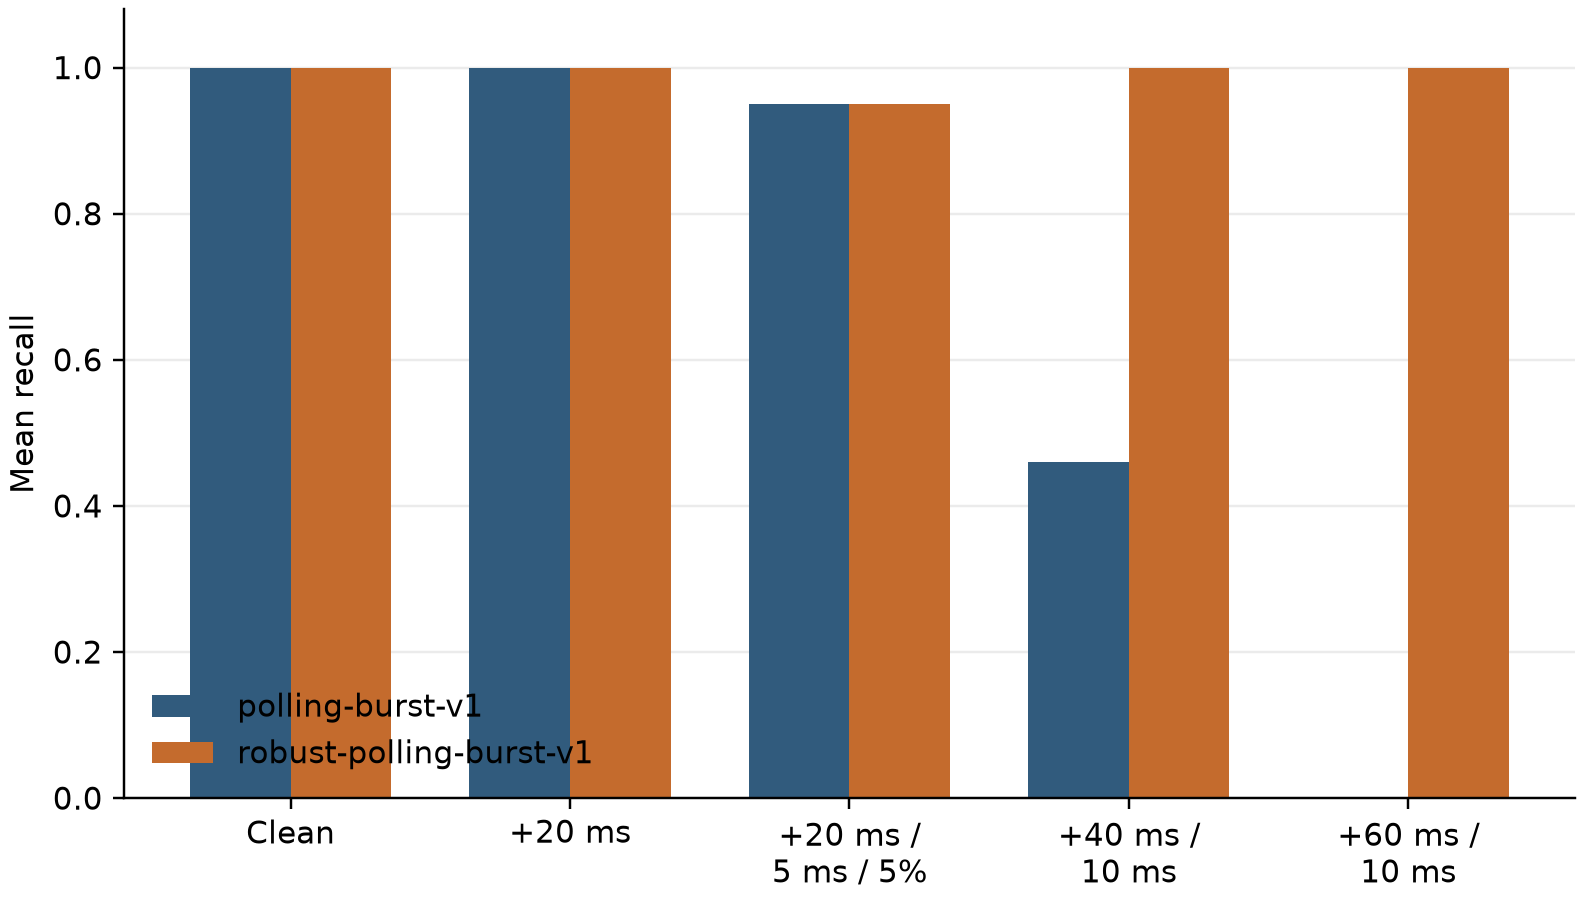
\includegraphics[width=.82\linewidth]{figures/recall_by_condition.png}
\caption{Mean recall by condition, read from the completed-study aggregate.}
\label{fig:recall}
\end{figure}

\begin{figure}[t]
\centering
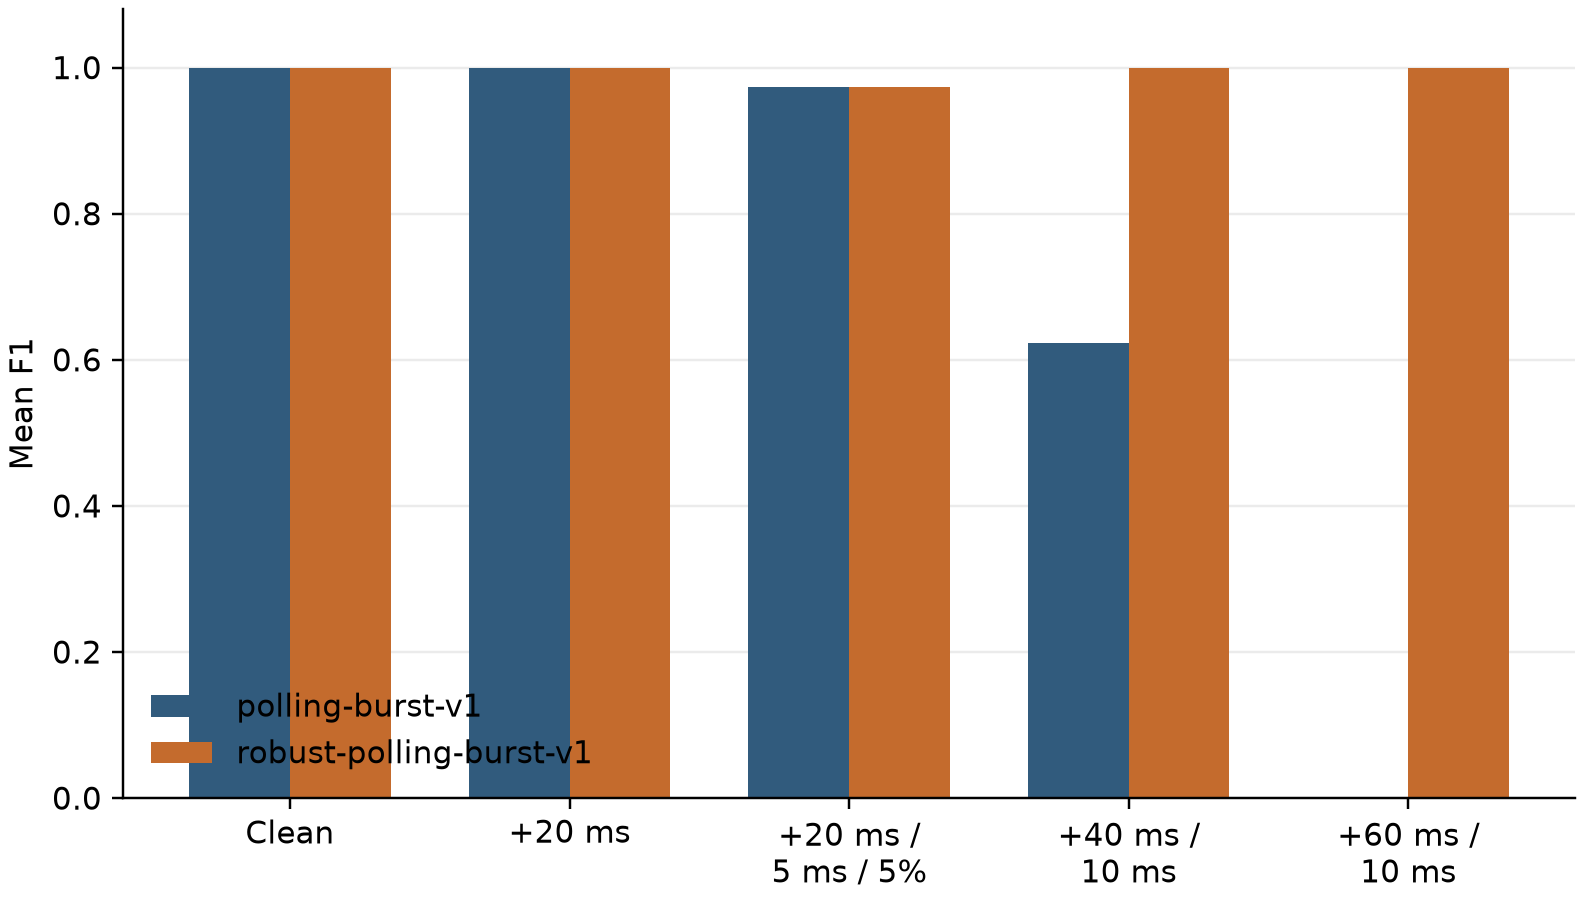
\includegraphics[width=.82\linewidth]{figures/f1_by_condition.png}
\caption{Mean run-level F1 by condition. F1 is averaged over runs, not recomputed from mean recall.}
\label{fig:f1}
\end{figure}

\section{Statistical and paired analysis}
For every detector and condition, the aggregate retains $N=25$, arithmetic mean,
sample standard deviation, minimum, maximum, and two-sided 95\% Student-$t$
intervals. Intervals use the 25 trial-level observations and are retained as
unbounded mathematical intervals. Paired effects are calculated within each run
as robust minus baseline and then summarized over the 25 differences; the 7,500
transactions are not treated as independent interval units.

The paired recall difference is 0 in the first three conditions, 0.54 at
Delay40/Jitter10 (95\% interval 0.4962180999417499--0.5837819000582501), and
1.0 at Delay60/Jitter10. The paired F1 mean is 0.3769897545292429 at Delay40
and 1.0 at Delay60. These are absolute run-level differences, not relative
percentages or population-wide effects; no multiplicity adjustment is claimed.

\begin{figure}[t]
\centering
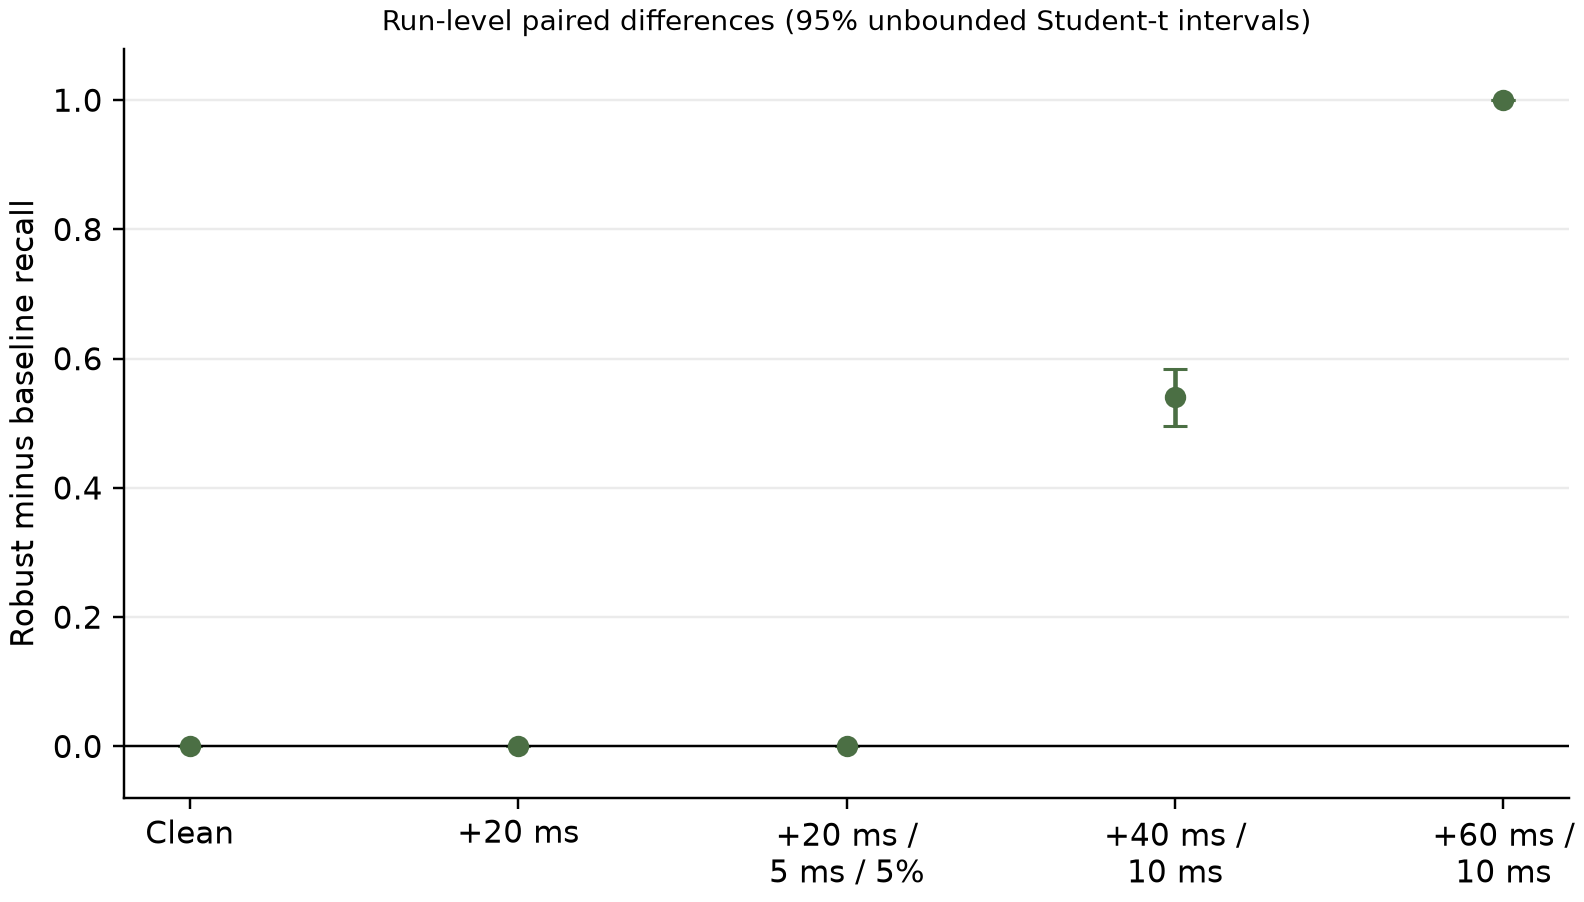
\includegraphics[width=.82\linewidth]{figures/paired_recall_difference.png}
\caption{Paired robust-minus-baseline recall differences and unbounded 95\% Student-$t$ intervals.}
\label{fig:paired}
\end{figure}

\section{Resource-cost measurement}
The evaluation retains prediction CPU time, wall-clock time, and traced peak
memory for each detector. These are small, host-specific measurements of the
evaluation step; they omit capture, container, operating-system, and deployment
cost. The aggregate is the source for the plotted means. They should not be
interpreted as total OT deployment cost or as a cross-host benchmark.

\begin{figure}[t]
\centering
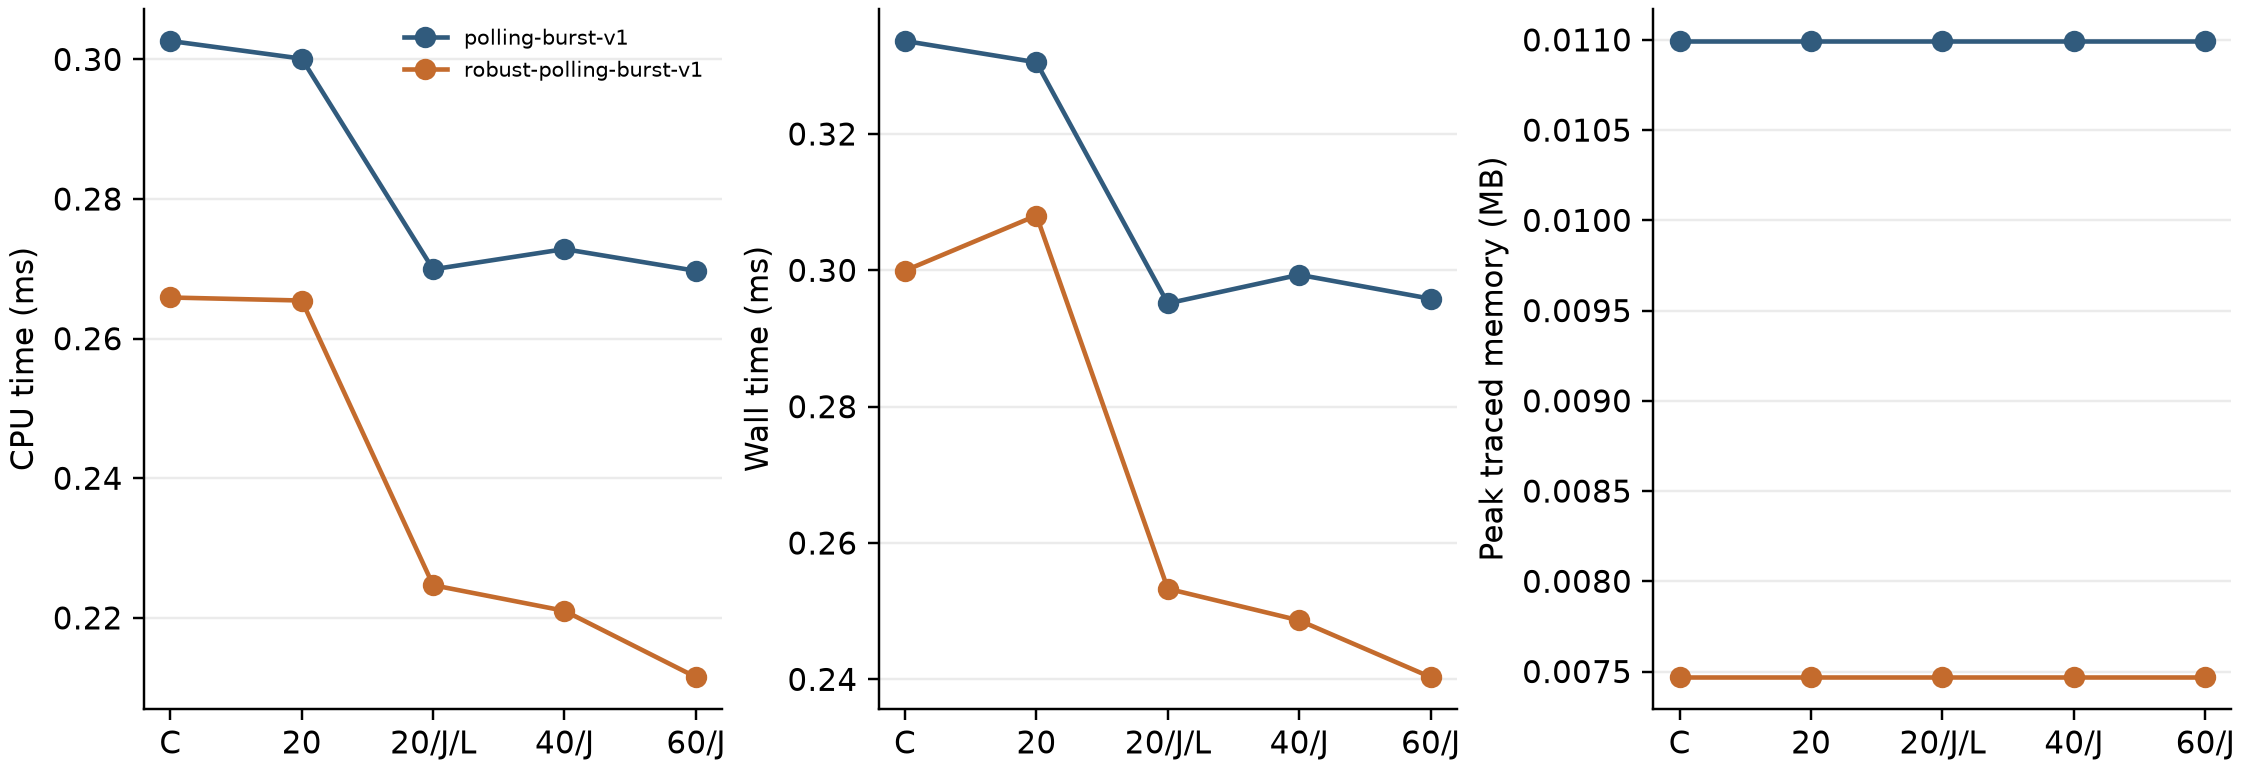
\includegraphics[width=.98\linewidth]{figures/resource_cost.png}
\caption{Recorded detector-evaluation resource metrics. Values are aggregate means; the source does not measure full deployment cost.}
\label{fig:resources}
\end{figure}

\section{Reproducibility}
All manuscript figures are generated from committed aggregate data by
\texttt{python paper/generate\_figures.py}. Software verification is
\texttt{./scripts/verify\_release.sh}, which performs whitespace checks, the
complete test suite, and a package build without launching Docker or OpenPLC.
The release package, source paths, study identifier, calibration hash, and
integrity manifest are listed in Appendix~\ref{app:reproducibility}. The
repository release is archived as \cite{palle2026otshield}.

\section{Threats to validity}
The experiment uses one isolated OpenPLC setup and one documented host
environment. Repeated trials on one host do not establish site-level or
cross-host independence. Server-side capture measures traffic arriving at that
observation point; another placement could yield different timing and visibility.
Student-$t$ intervals are descriptive run-level summaries for bounded metrics,
with no population or multiplicity claim. The mutable image tag alone is not a
complete environment specification, so the retained image identity and per-run
provenance matter.

\section{Limitations}
The workload is read-only \fc{} traffic and a polling-burst anomaly. The study
does not evaluate write operations, other Modbus functions, DNP3, EtherNet/IP,
full GRFICSv3 process simulation, production networks, or independent external
replication. It measures detector behavior under the tested delay, jitter, and
loss values, not all degraded-connectivity regimes. Synthetic fixtures are
useful software tests but are not additional laboratory evidence.

\section{Discussion}
The results show why coverage and timing-based effectiveness should be reported
together. In the heavier tested delay conditions, the robust threshold preserved
the burst signal while the fixed 50~ms threshold lost recall; this is a specific
observation for the documented setup, not evidence of universal detector
superiority. The paired design, frozen calibration, explicit run units, and
failure preservation make the result auditable. The earlier duplicate-TID and
infrastructure failures remain disclosed and excluded from the replacement
aggregate; they were not silently pooled or used to tune the threshold.

\section{Conclusion}
\otb{} v0.6 provides a reproducible measurement package for OT detection
resilience under controlled connectivity impairment. In the completed isolated
OpenPLC study, the independently calibrated detector matched the baseline in
clean and lighter conditions and retained recall under the heavier tested delay
conditions. The principal result is methodological: a frozen, paired,
evidence-preserving workflow can separate observation coverage from timing-based
detection resilience while keeping claims bounded to the measured laboratory.

\section{Reproducibility and data availability statement}
The software and completed evidence are available in the GitHub repository and
the archived \texttt{v0.6.0-alpha} release at Zenodo DOI
\url{https://doi.org/10.5281/zenodo.22899466}. The committed evidence root,
manifest, calibration file, protocol, errata, and source code support analysis
reproduction. Reproducing the figures and aggregate interpretation requires no
laboratory execution. Any future laboratory reproduction must use an authorized,
isolated environment and the bounded read-only protocol; readers must not send
traffic to real OT systems.

\bibliographystyle{plain}
\bibliography{references}

\appendix
\section*{Reproducibility appendix}
\label{app:reproducibility}

The software is archived as OTShield Bench \texttt{v0.6.0-alpha} at
\url{https://github.com/ASHTHRA/otshield-bench/releases/tag/v0.6.0-alpha} and
Zenodo DOI \url{https://doi.org/10.5281/zenodo.22899466}. The repository is
\url{https://github.com/ASHTHRA/otshield-bench}. The release declares Python
package version \texttt{0.6.0a0}; the completed study provenance records Python
3.14.4, Docker 29.8.1, Compose v5.5.1, and the Linux/WSL2 kernel used for the
isolated laboratory run.

The repository's software CI runs on Ubuntu and Windows with Python 3.10 and
3.12. POSIX-only v0.6 lifecycle tests are explicitly skipped on native Windows;
portable package, analysis, and accounting tests remain cross-platform. The
manuscript workflow additionally compiles this file and \texttt{main.tex} with
TeX Live in GitHub Actions and uploads the resulting PDF as a workflow artifact.

The study identifier is \texttt{20260922T021855Z}. Its source files are
\texttt{evidence/v06/20260922T021855Z/aggregate.json} and
\texttt{evidence/v06/20260922T021855Z/study.json}; per-run captures and
provenance are under the same evidence root. The release manifest and
\texttt{STUDY\_SHA256SUMS} provide integrity records. The frozen calibration is
\texttt{research/v0.6\_calibration.json}, whose recorded SHA-256 is
\texttt{d8676d4670ba44c0f4b1045e5e07dd2d251ccb4a63ed8089b9b9aada729ea234}.

Software verification is performed with:

\begin{verbatim}
./scripts/verify_release.sh
python paper/generate_figures.py
\end{verbatim}

The first command checks whitespace, runs the complete test suite, and builds
the package. The second reads only committed aggregate data and deterministically
writes the figures in \texttt{paper/figures/}. These commands reproduce the
analysis and manuscript artifacts; they do not launch Docker, OpenPLC, packet
capture, or laboratory traffic.

The figures intentionally read the aggregate rather than duplicating numerical
constants in plotting code. Their condition labels and detector names are the
declared v0.6 schema values; all metric means and interval endpoints come from
\texttt{aggregate.json}. The manuscript's prose is a human-readable rendering
of the same bounded result set and the technical report.

Reproducing the laboratory measurements is a separate activity requiring an
explicitly authorized, isolated Linux/Docker environment. The protocol uses
bounded read-only Modbus/TCP Function Code 3 requests and must never be aimed at
a real operational system. The preserved failed attempts and errata remain in
the repository and are excluded from the completed replacement aggregate.


\end{document}
